\documentclass[12pt]{article}
\usepackage[utf8]{inputenc}
\usepackage{upquote}
\usepackage[margin=1in]{geometry} 
\usepackage{amsmath,amsthm,amssymb}
\usepackage{graphicx}
\usepackage{listings}
\newenvironment{statement}[2][Statement]{\begin{trivlist}
\item[\hskip \labelsep {\bfseries #1}\hskip \labelsep {\bfseries #2.}]}{\end{trivlist}}
\usepackage{booktabs}
\usepackage{multirow}
\usepackage{subfigure}


% Listings package for code rendering (No external dependencies)
\usepackage{listings}  
\usepackage{xcolor}   % Color support
\usepackage{tcolorbox} % Box for better appearance

% Define custom colors for code highlighting
\definecolor{codegreen}{rgb}{0,0.6,0}
\definecolor{codegray}{rgb}{0.5,0.5,0.5}
\definecolor{codepurple}{rgb}{0.58,0,0.82}
\definecolor{backcolour}{rgb}{0.95,0.95,0.92}


\lstset{frame=tb,
    language=Python,
    backgroundcolor=\color{backcolour},   
    commentstyle=\color{codegreen},
    keywordstyle=\color{magenta},
    numberstyle=\tiny\color{codegray},
    stringstyle=\color{codepurple},
    basicstyle=\ttfamily\footnotesize,
    breakatwhitespace=false,         
    breaklines=true,                 
    keepspaces=true,                 
    numbers=left,       
    numbersep=5pt,                  
    showspaces=false,                
    showstringspaces=false,
    showtabs=false,                  
    tabsize=2,
}


\title{Handin 2}

\begin{document}
\maketitle

\section{Introduction}

We investigate the implementation and benchmarking of the Steepest Descent and Newton's Method, both using backtracking line search. We aim to analyze their convergence behavior and compare their efficiency.  We also solve theoretical problems that provide insights into the algorithmic choices and expected performance. 

In our benchmark protocol, we focus on the five functions provided in the case study. 

\section{Experiments Setup}

\subsection{Stopping Criteria}
% Discuss what stopping criteria you use and why? How do you pick the values for the stopping thresholds?
We apply two kinds of stopping criteria, including the gradient norm threshold and the maximum iteration threshold. We use the gradient norm threshold to ensure the algorithm stops when the gradient is sufficiently small. We use the max iteration to limit the algorithm to run infinitely when there is ill conditions, in case the algorithm would run definitely.

\begin{lstlisting}
# Max Iteration Number
for _ in range(max_iter): 
    grad = grad_f(x)
    # Gradient Norm Threshold 
    if np.linalg.norm(grad) < tol:
        break
\end{lstlisting}

\textbf{Stopping Threshold Value Choice: }We choose the tolerance gradient value=1e-6 because it is small enough and will not cost too much iterations. We choose max iterations=10, because the gradient norm threshold will reach firstly in our experiment, so the max iterations will not effect the gradient norm threshold. 

\subsection{Parameter Selection }
% How do you select parameter values for the backtracking line search? Is your result sensitive towards these settings?
Here we discuss our parameter selections and their logic in Backtracking Line Search. As the Armijo issues:

\begin{equation}
\begin{aligned}
if \, & f(x_k + \alpha d_k) \leq f(x_k) + c_1 \alpha \nabla f(x_k)^T d_k:\\
& \alpha = \rho * \alpha
\end{aligned}
\end{equation}

There are 3 selectable variables in Backtracking Line Search, as listed below. The initial searching point $x_0$ also matters, but we will not discuss much since we have done this in hand-in1. So we directly use the selection of $x_0$ from hand-in1's conclusion.

\begin{enumerate}
  \item The initial step size $\alpha_0$: we unify $\alpha_0$ to 1.0.
  \item The sufficient decrease parameter $c_1$: we unify $c_1$ to $1e-4$.
  \item The step shrinking factor$\rho$: we select different $\rho$, from ${0.1,0.3,0.5,0.9}$.
\end{enumerate}

\subsubsection{Selection of $\alpha_0$}
We consider the $\alpha_0$ choice based on the different step scales in Newton's and Steepest Decent algorithm.

For Newton's method, since Hessian is considered in the step direction, it can choose a naturally satisfying-Armijo-condition step when the Hessian is well-conditioned. The function decrease is typically large enough that $\alpha_0=1.0$ satisfies the Armijo condition without backtracking. When the Hessian is ill-conditioned, backtracking is required, and $\alpha$ wii reduce.

For Steepest Decent, the search direction does not consider the second-order information, so the step size is often poorly scaled. A full step like $\alpha_0=1.0$ may fail to satisfy the Armijo condition. But it just lead to a few more back tracking, so for convenience we just unify the $\alpha_0=1.0$ in our benchmark protocol.

\subsubsection{Selection of $c_1$}

The parameter $c_1$ controls how much decrease is required in $f(x)$ per step. A smaller $c_1$  would require a more significant decrease, leading to excessive shrinking of $\alpha$ and slower convergence. A larger $c_1$ would accept even small improvements and might allow larger steps, but this could lead to instability.

For Newton's Method, the step is well-scaled when the Hessian is well-conditioned, and the Armijo condition is often easily satisfied. So Newton's Method is less sensitive to $c_1$.

For Steepest Descent, it is sensitive to $c_1$'s choice. Because its gradient steps are poorly scaled, so $c_1$ cannot be too large. $1e-4$ is a common choice among the standard library, for example, in scipy.optimization.line\_search. 

Since the two algorithms could reach a common need for $c_1$, we just unify the $c_1$ in the benchmark protocol to $1e-4$.

\subsubsection{Selection of $\rho$}

For Newton's Method, backtracking is rarely needed when the Hessian is well-conditioned, and when backtracking is required, a larger $\rho$ is preferred because Newton's step is often in the right direction, and only small adjustment is needed.

For Steepest Descent, since it often produces steps that violate the Armijo condition, backtracking is frequently needed. A larger $\rho$ makes the step size shrink slowly, leading to more backtracking iterations. So a smaller $\rho$ is preferred, so that the $\alpha$ could shrink quickly.

Since the two algorithms have different preference to $rho$, and both of them are somehow sensitive to the $\rho$, our benchmark protocols covers different $\rho$. 

\section{Results and Discussion}

Our benchmark protocol cover the following two features: 

\begin{enumerate}
  \item Different target functions, particularly the functions provided in the case\_study.py;
  \item Different backtracking step lengths($\rho$).
\end{enumerate}

\subsection{Correctness Verification}
% Evaluate whether your results are correct. Describe the steps you took to ensure correctness of your algorithms and show data that supports your claims.

\textbf{Step1} We print logs to see the Hessian and gradient calculation during the iterations, so that we can see whether the Hessian is ill-condition(near singular) or not.

\textbf{Step2} We also have numerical methods to prove the correctness, printed in the log. These include the convergence rate, step sizes and final error. 


\subsection{Step Length Observations}
% For both algorithms, describe your observations of the chosen step lengths. Are there important differences between the functions and algorithms?
Newton is not sensitive to the chosen step lengths when the Hessian is well-conditioned and in this case all step length choices behaves the same(see $f_1$, $f_3$, $f_4$, $f_5$). When Hessian is ill-conditioned, backtracking is needed, and different $\rho$ leads a slight different behavior. But all of the step length choices still behave similarly.

For Steepest Descent, we will discussion according to the functions one by one. We also discover the relationship of convergence speed cannot be linear related to the value of $\rho$. For example, the convergence speed may be $\rho=0.3<\rho=0.1<\rho=0.9<\rho=0.5$.

For f1, the step length varies with $\rho=0.3$ achieves the fastest convergence, more specifically the iteration number $\rho=0.3<\rho=0.1<\rho=0.9<\rho=0.5$. 
For f2, the step length varies with $\rho=0.9$ achieves the fastest convergence, with 1 iteration and reach a optimization. Others miss the optimized solution, and converge slowly. 
For f3, the $\rho=0.5$ and $\rho=0.3$ can reach a convergence but not the optimized, while the $\rho=0.1$ and $\rho=0.9$ reaches a stagnation.
For f4, $\rho=0.5$ reaches the optimization in 1 iterations. Others also can reach a optimization, but much slower, and $\rho=0.9$ has a zig-zag.
For f5, all can reach a optimization, while different iterations required, typically $\rho=0.5 < \rho=0.1 \approx \rho=0.3 < \rho=0.9$.

\subsection{Convergence Plots and Analysis}
% Show convergence plots and based on the empirical results, state whether the algorithms likely have Q-linear, Q-superlinear or maybe even Q-quadratic convergence on the different functions.

The convergence plots is shown in Figure~\ref{fig:convgraph}. 

For f1, Newton's method vertically reaches optimum in 1 iteration, and it shows a Q-quadratic convergence. Steepest Descent  shows a slower convergence and it is a Q-Linear convergence.

For f2, it is complicated. For Newton’s Method it looks only Q-super-linear, because the Hessian is ill-conditioned. For Steepest Descent, when the $\rho$ is as large as 0.9, it shows a Q-quadratic convergence. When $\rho$ is smaller(0.1,0.3,0.5), it behaves like Q-Sub-Linear. Here these $\rho$ may be too small, leading to numerical stagnation.

For f3, we select a initial $x_0$ to make sure the Hessian function is well-conditioned(other $x_0$ may lead to stagnation in Newton's Method). So the Newton's Method is Q-quadratic. For Steepest Descent, it reaches stagnation, suggesting the step length may be missing the optimized solution, showing Q-Sub-Linear.
% $\rho=0.1$ and $\rho=0.9$ 

For f4, Newton's method vertically reaches optimum in 1 iteration, and it shows a Q-quadratic convergence. Steepest Descent is Q-Linear.

For f5, Newton's method and Steepest Descent are all Q-Linear.

\begin{figure}[ht]
\centering
\subfigure[]{
    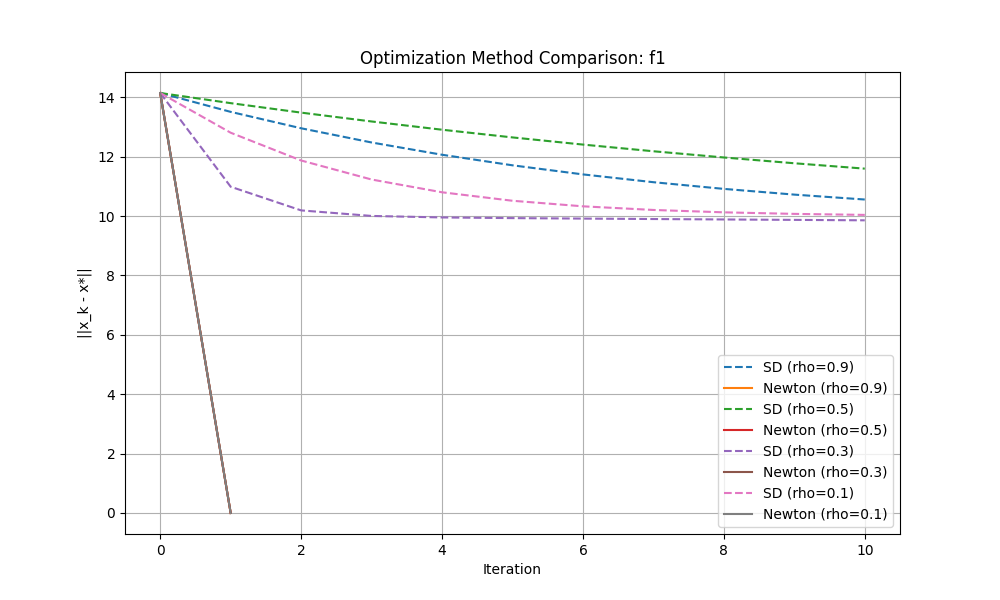
\includegraphics[width=0.15\columnwidth, keepaspectratio]{pics/w2-f1}
\label{fig:f1}
}
\subfigure[]{
    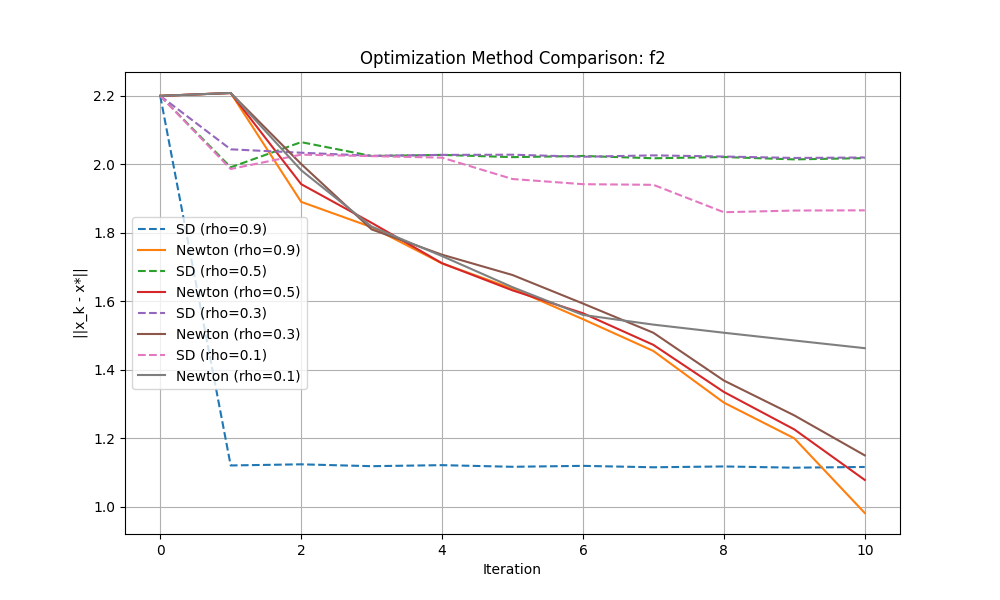
\includegraphics[width=0.15\columnwidth, keepaspectratio]{pics/w2-f2}
    \label{fig:f2}
}
\subfigure[]{
    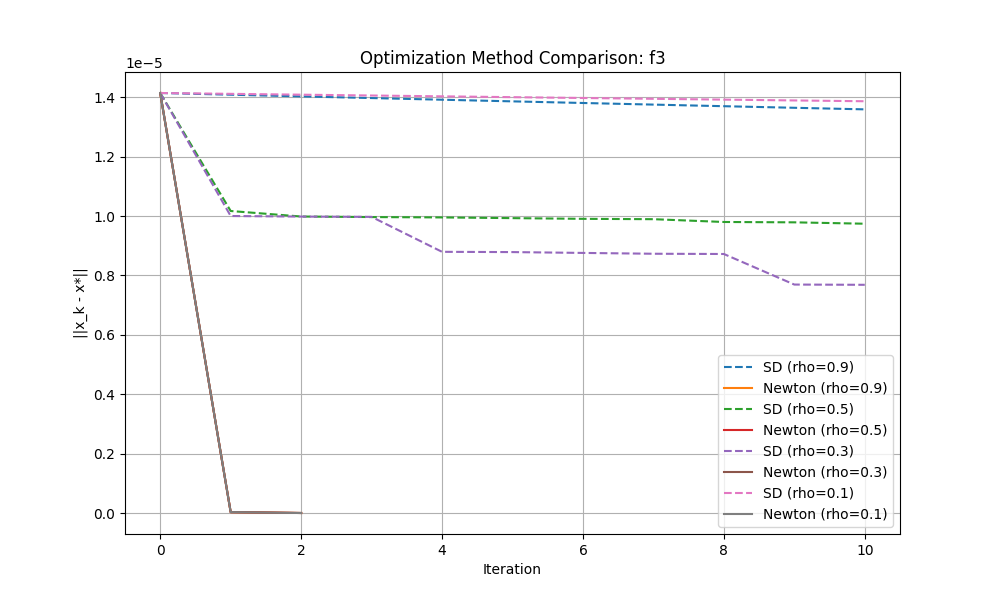
\includegraphics[width=0.15\columnwidth, keepaspectratio]{pics/w2-f3}
    \label{fig:f3}
}
\subfigure[]{
    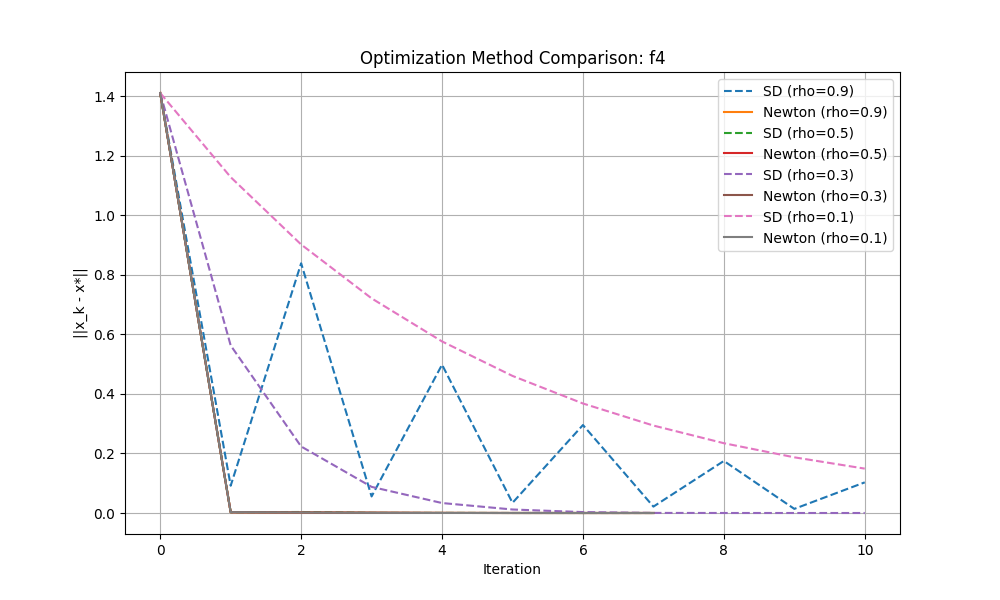
\includegraphics[width=0.15\columnwidth, keepaspectratio]{pics/w2-f4}
    \label{fig:f4}
}
\subfigure[]{
    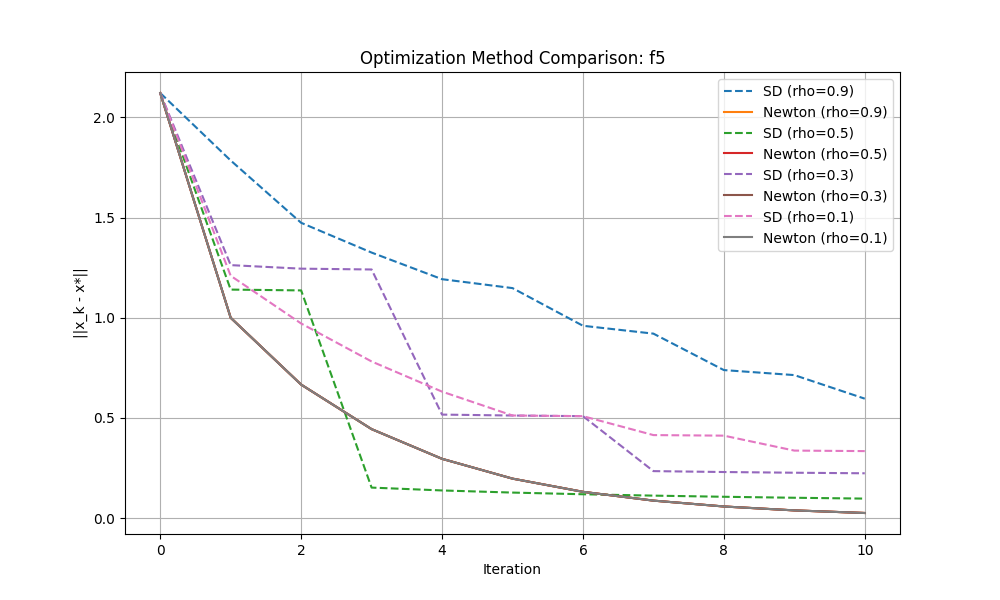
\includegraphics[width=0.15\columnwidth, keepaspectratio]{pics/w2-f5}
    \label{fig:f5}
}
\caption[]{Convergence graph(log scale) of the three optimize algorithms on the five functions, analyzing iterations}
\label{fig:convgraph}
\end{figure}


\section{Theory}

\subsection{Question 1: Sum of Different Powers Function}
% TODO 

\subsection{Question 2: Sufficient Decrease Condition in 1D}
% TODO 

\section{Conclusion}
% TODO 

\end{document}
